% vim: spell spelllang=es:
\documentclass[12pt, oneside]{article}
\usepackage[a4paper, left=2.5cm, right=2.5cm, top=2.5cm, bottom=2.5cm]{geometry}

\usepackage[utf8]{inputenc} % Use unicode
\usepackage[T1]{fontenc}
\usepackage[spanish,es-tabla]{babel} % Names in spanish


\usepackage{xcolor}
\usepackage{siunitx}

%% Bibliography:
%\usepackage{comment}
%\usepackage[
    %backend=biber,
    %style=numeric,
%]{biblatex}
%\DeclareNameAlias{default}{last-first}

%\usepackage{csquotes}       % For bibliography quotations
%\DeclareQuoteAlias{spanish}{catalan}

%\addbibresource{biblio.bib}
%% see:
%% https://www.sharelatex.com/learn/Bibliography_management_in_LaTeX#The_bibliography_file

%\usepackage{datetime} % Customize date
%% \monthyeardate\today gives the date without the day
%\newdateformat{monthyeardate}{%
    %\monthname[\THEMONTH], \THEYEAR}

% For cross references
\PassOptionsToPackage{hyphens}{url}\usepackage[colorlinks = true]{hyperref}
\usepackage[catalan]{varioref}
%\usepackage{cleveref}
%hyperref configuration so that it doesn't contrast so much colorlinks,
\hypersetup{
   linkcolor={black},
   citecolor={black},
   %linkcolor={red!50!black},
   %citecolor={blue!50!black},
   urlcolor={blue!80!black}
}

\usepackage{mathtools}  % amsmath + more
\usepackage{amsthm}     % Theorem enviroment
\usepackage{amssymb}    % More symbols
\usepackage{amstext}    % Text inside mathenv

\usepackage{relsize}    % Bigger math with mathlarger{___}
\usepackage{nicefrac}   % nice fractions in one line

\usepackage[export]{adjustbox}  % Adjust table size
\usepackage{float}              % Force tables and images position (H and H!)
\usepackage{wrapfig}            % Wrap images like in HTML

\usepackage{tabularx, colortbl, booktabs}    % Better tables
\usepackage{longtable}                      % Multiple page table

% Split cell in lines and more formating options inside table
\usepackage{array, multirow, multicol, makecell}

%\usepackage{subcaption}                     % Subfigures
%\usepackage[framemethod=tikz]{mdframed}     % Custom frames

%\usepackage[bottom]{footmisc} % Footnotes at bottom of page

%\usepackage[alsoload=hep]{siunitx}          % SI units and uncertainties
%\sisetup{locale = FR}                       % Commas and so on for spanish
%\sisetup{separate-uncertainty=true}
%\sisetup{
  %per-mode=fraction,
  %fraction-function=\nicefrac
%}

%\usepackage{tikz}
%%\usetikzlibrary{arrows}
%%\usetikzlibrary{scopes}
%\usetikzlibrary{babel}

%\usepackage{listings}       % For code blocks

%% Custom code highlight
%\definecolor{codegreen}{rgb}{0,0.6,0}
%\definecolor{codegray}{rgb}{0.5,0.5,0.5}
%\definecolor{codepurple}{rgb}{0.58,0,0.82}
%\definecolor{backcolour}{rgb}{0.95,0.95,0.92}
%\definecolor{lightblue}{RGB}{135,206,250}

%\lstdefinestyle{mystyle}{ backgroundcolor=\color{backcolour},
    %commentstyle=\color{codegreen}, keywordstyle=\color{blue},
    %numberstyle=\tiny\color{codegray}, stringstyle=\color{red},
    %identifierstyle=\color{black}, basicstyle=\footnotesize,
    %%breakatwhitespace=false,
    %breaklines=true,
    %%captionpos=b,                    keepspaces=true,
    %numbers=left,                    numbersep=5pt,
    %showspaces=false,
    %%showstringspaces=false, showtabs=false,
    %tabsize=4
%}
%\lstset{style=mystyle}

\newcommand{\whitepage}{
    \clearpage\thispagestyle{empty}\addtocounter{page}{-1} \newpage \clearpage
}

% Add command before appendix session for page numbering: A-1
%\newcommand{\appendixpagenumbering}{
    %\break
    %\pagenumbering{arabic}
    %\renewcommand{\thepage}{\thesection-\arabic{page}}
%}

%% Custom Math operators (functions not in italic in math mode):
%\DeclareMathOperator{\arcsec}{arcsec}
%\DeclareMathOperator{\arccot}{arccot}
%\DeclareMathOperator{\arccsc}{arccsc}
%\DeclareMathOperator{\cis}{cis}


\usepackage[bottom]{footmisc}

\usepackage{amsmath}
\usepackage[justification=centering]{caption}

\title{%
IA: Trabajo de innovación
}

\author{%
    Aleix Boné\\
    Alex Herrero\\
    Moisés Balcells
}
\date{%
Mayo 2020
}

\begin{document} 


\thispagestyle{empty}
\clearpage
\setcounter{page}{-1}

\begin{titlepage}
{
    \centering
    \null
    \vfill
    {\Large Inteligencia Artificial\par}
    \vspace{2em}
    {\Huge 
    Trabajo de innovación \\
    \par}
    \vspace{1em}
    {\Huge\bfseries 
    AIRx\textsuperscript{\texttrademark}
    \\ Intelligent MR slice prescription
    \par}
    \vspace{2em}
    {\large \scshape 
    Mayo 2020
    \par}
    \vfill
\begin{center}
    
\end{center}
    \vspace{3cm}

    \vfill
    {\raggedleft \large
Aleix Boné Ribó\\
Alex Herrero Pons\\
    Moisés Balcells
        \par}
}
\end{titlepage}

\pagebreak

\thispagestyle{empty}
\clearpage
\setcounter{page}{0}

\tableofcontents

\pagebreak

%\section{Trabajo de innovación}
%
%El tema sobre el que trabajaremos es el escaneo inteligente con deep learning aplicado a la resonancia magnética. 
%En este ámbito la inteligencia artificial se utiliza para hacer el escaneo de imágenes más preciso y rápido. 
%En concreto nos centraremos en el producto AIRx™ de general electric healthcare.

%     Descripción del producto o servicio
%     Descripción de las técnicas de IA que se han utilizado
%     Descripción de cómo han sido utilizadas las técnicas
%     Explicación de porqué es un producto/servicio innovador y la naturaleza de la innovación (innovación en la técnica/método de IA, uso innovador de técnicas ya existentes)
%     Impacto del producto en la empresa (beneficios, riesgos, posición en el mercado)
%     Impacto del producto en el usuario o en la sociedad (beneficios y riesgos)
%      Bibliografía/Referencias utilizadas para la elaboración del documento

\null
\vspace{4em}

\section{Introducción}
Actualmente, en el campo de la medicina hay diversas técnicas para observar alteraciones en los tejidos y detectar cáncer y otras patologías. Una de las técnicas más conocidas y utilizadas es el análisis de imágenes creadas por resonancia magnética (MRI). 

La MRI es una técnica no invasiva utilizada en radiología que hace uso del fenómeno de la resonancia magnética nuclear para extraer información sobre la estructura y composición del cuerpo a analizar. Seguidamente esta información es procesada y transformada en imágenes mediante un proceso informático. Estas imágenes además de representar estructuras anatómicas, también son capaces de representar fisiología y función como por ejemplo el flujo sanguíneo o la perfusión y difusión.

A pesar de que su principal aplicación es en el campo de la medicina, esta técnica también es utilizada en el campo de la industria para analizar la estructura de materiales tanto orgánicos como inorgánicos.

El proceso de interpretar la información extraída y convertirla en imágenes ha mejorado drásticamente en la última década gracias a las CNNs, un tipo de redes neuronales que explicaremos más adelante.

\pagebreak
\section{Descripción del producto}
La empresa GE Healthcare dispone de una familia de productos llamada AIR destinados exclusivamente a mejorar la resonancia magnética mediante la inteligencia artificial. En concreto nosotros hablaremos de AIRx, un producto que incorpora el Deep Learning para obtener imágenes de MRI mediante la segmentación en planos y el uso de las CNNs.
% TODO: https://www.gehealthcare.com/products/magnetic-resonance-imaging/air-technology
% ñe, a ver que te parece, no sé si es esto la verdad

% TODO: meter esto ?? where, que link es?
%dale en el doucmento generado para verlo
% www.gesignapulse.com/signapulse/autumn_2018/MobilePagedArticle.action?articleId=1444512
% es una puta mierda, no dice nada en verdad... XD
\cite{noauthor_introducing_nodate}

    \subsection{\emph{Magnetic Ressonance Imaging} (MRI)}%
     %\footnote{Imagen por Resonancia Magnética (IRM)} 
    En el examen de MRI, el operador de exploración primero adquiere un conjunto de imágenes de "localizador" de baja resolución (figura~\ref{fig:resonancia}) a partir de las cuales se puede identificar la ubicación y orientación aproximadas de los puntos de referencia deseados. Estas referencias anatómicas se utilizan para planificar manualmente las ubicaciones exactas, la orientación y la cobertura requerida para las imágenes que se utilizarán para los escaneos de alta resolución que se utilizan para el diagnóstico. Este procedimiento es complicado ya que la orientación, la ubicación y la cobertura deben ser correctas en las tres dimensiones
     espaciales.
     
     \begin{figure}[H]
        \centering
        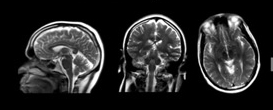
\includegraphics[width=0.9\textwidth]{resonancia.png}
        \caption{Ejemplo de 3 cortes distintos obtenidos mediante MRI}%
        \label{fig:resonancia}
     \end{figure}
    
    La calidad y la consistencia del posicionamiento y la orientación de los cortes
    \footnote{Un corte es el plano espacial en el que se realiza el escaneo (\emph{slice})}
    depende en gran medida de la habilidad y experiencia del operador de escaneo. Este proceso puede llevar mucho tiempo y ser difícil, especialmente para las anatomías complejas. Como resultado, puede haber inconsistencias de un operador de escaneo a otro. Esta falta de consistencia puede hacer que el trabajo del radiólogo al interpretar estas imágenes sea más difícil, especialmente cuando un paciente está siendo escaneado como un seguimiento de un examen de resonancia magnética anterior y están tratando de identificar cambios sutiles en la anatomía o la progresión de la enfermedad con el tiempo. En el peor de los casos, no se obtienen las imágenes correctas y el paciente debe regresar para otro procedimiento.
    
    \subsection{Antecedentes}
    
    El uso de técnicas de IA en medicina esta muy extendido y se pueden encontrar muchos ejemplos en muchas áreas de la medicina. En el campo
    de los MRI se han hecho varios estudios sobre el uso de CNNs para hacer diagnósticos a partir de imágenes MRI \cite{bien_dont_2018,noauthor_deep-learning_nodate}. Un ejemplo es un estudio
    sobre la detección de cáncer metastático en imágenes MRI \cite{grovik_deep_2020}.
    Sin embargo la mayoría de los estudios realizados se centran en el diagnostico, AIRx busca agilizar el proceso de toma de las imágenes
    que se usaran para el diagnostico.
    
    \subsection{AIRx}
    
    % TODO
    
    El módulo AIRx incorpora tecnología CNN, a este módulo el tiempo que le toma al operador de exploración determinar las ubicaciones y orientaciones para los cortes de exploración deseados para una resonancia magnética cerebral puede reducirse entorno al 40-60 por ciento. Y además gracias a este módulo se puede ver una reducción en los errores y una precisión mejorada. Esto se puede traducir como  resultados de exámenes generales más cortos,con una posibilidad reducida de devolución de llamadas del paciente y una mejor calidad de diagnóstico del examen.

\pagebreak
\section{Técnicas de IA}

    \subsection{Convolutional Neural Networks (CNN)}
    
    Las redes neuronales convolucionales son un caso especifico de redes neuronales de deep learning
    en las que la entrada son imágenes. Una CNN consiste en varias capas de convolucion y subsampling (o pooling)
    que extraen las características (\emph{features}) de la imagen que se usan como entrada de una \emph{fully connected layer}
    que clasifica la imagen \cite{saha_comprehensive_2018,noauthor_deep_nodate,noauthor_hackfromhome_nodate}.
    En la figura~\ref{fig:cnn} se muestra un esquema de la estructura de una CNN.
    
     \begin{figure}[H]
        \centering
        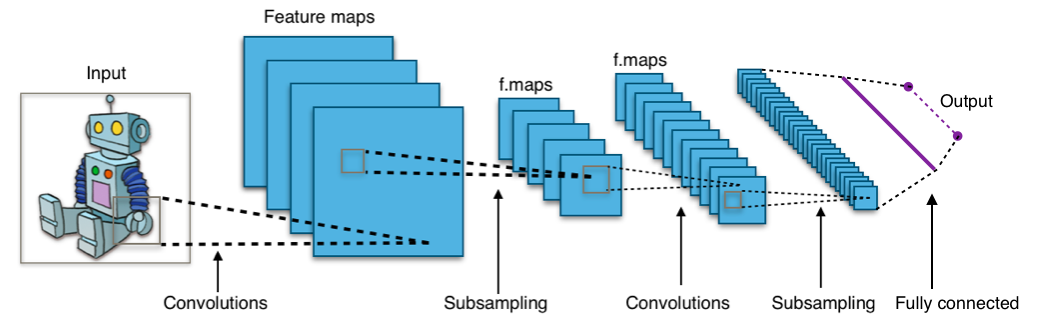
\includegraphics[width=0.9\textwidth]{cnn}
        \caption{CNN \cite{aphex34_english_2015} }%
        \label{fig:cnn}
     \end{figure}
    
    \subsection{U-net}
    
    U-net es un tipo de CNN para la segmentación de imágenes, es decir dividir la imagen inicial en
    segmentos. Se basa en la aplicacion de una CNN de classificacion y una vez llegada a la salida de
    classificacion, usar-la como entrada junto con los datos de los pasos anteriores deshaciendo los
    pasos de pooling hasta llegar a producir una salida que segmenta la imagen según la característica.
    La figura~\ref{fig:unet} ilustra un ejemplo de U-net en la que se puede observar como se usan
    los resultados de la classificacion y los \emph{featrure maps} de cada nivel de pooling para
    generar la salida.(se puede apreciar también la forma de U del diagrama que da el nombre a la red).
    
     \begin{figure}[H]
        \centering
        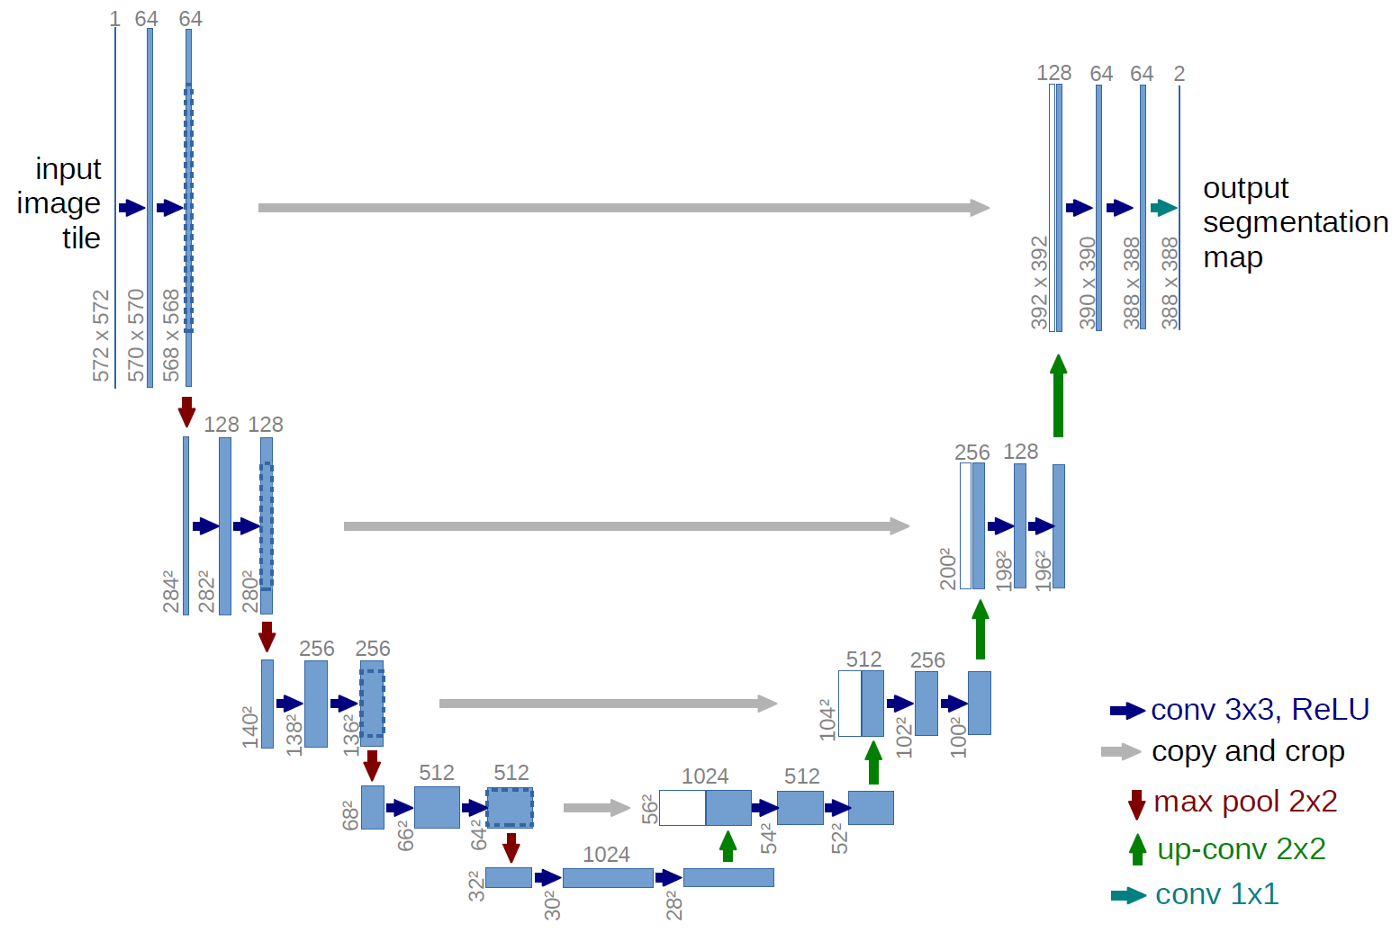
\includegraphics[width=0.7\textwidth]{unet}
        \caption{Arquitectura U-net \cite{sankesara_u-net_2019}}%
        \label{fig:unet}
     \end{figure}
     
\pagebreak
\section{Uso de las técnicas de IA}

    El proceso se divide en 3 etapas \cite{noauthor_ge_nodate-1}:
    \emph{LocalizerIQ-Net}, \emph{Coverage-Net} y \emph{Orientation-Net}, cada una de ellas usa varias 
    CNNs distintas.

     \begin{figure}[H]
        \centering
        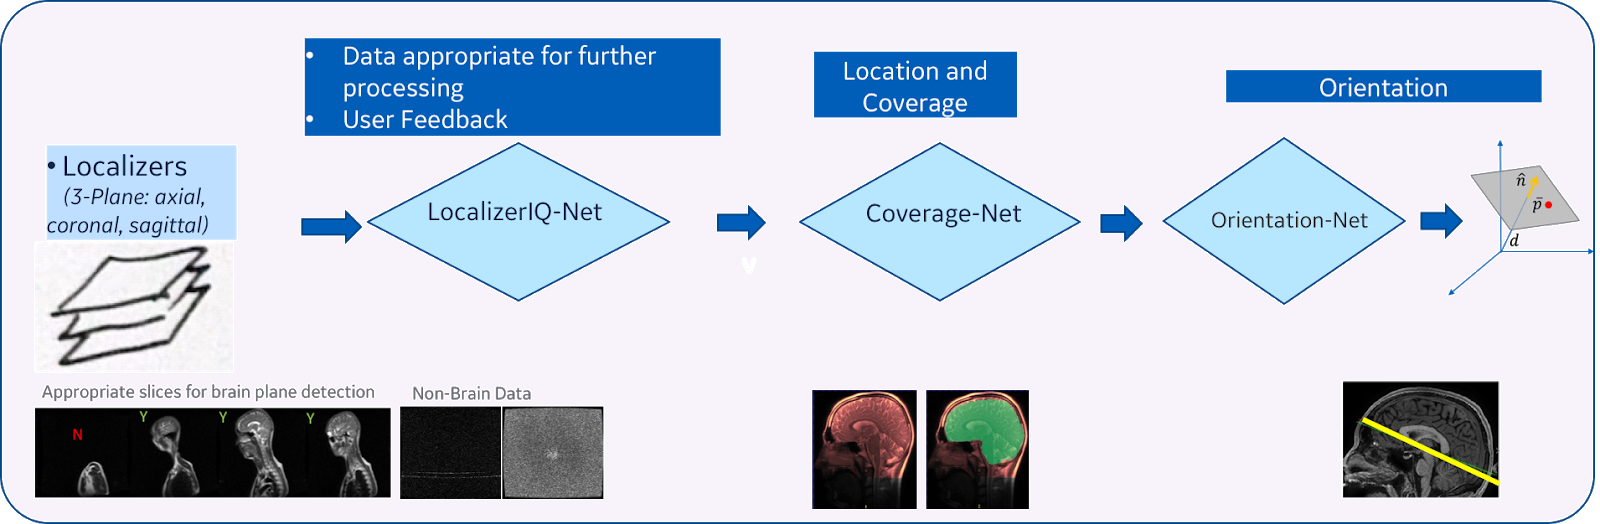
\includegraphics[width=0.9\textwidth]{steps}
        \caption{Etapas \cite{noauthor_ge_nodate-1}}%
        \label{fig:steps}
     \end{figure}

    \subsection{LocalizerIQ-Net}
    
    Esta etapa decide para cada una de las imágenes de localización iniciales si es útil para
    identificar el corte de la anatomía deseada. Esto sirve para identificar si las imágenes iniciales
    son buenas y útiles para las siguientes fases o si el operador debe realizar mas escáneres.
    
    En esta etapa se usa una red neuronal convolucional de clasificación de 5 capas que clasifica
    las imágenes obtenidas como aptas o no.
    
    \subsection{Coverage-Net}
    
    Esta etapa se encarga de localizar la posición de la anatomía del paciente a analizar, en este caso
    el cerebro. Para ello se usa una U-net que segmenta la imagen identificando que parte de la imagen
    forma parte del cerebro. Esto permite que la siguiente etapa no dependa de cambios en la posición del
    paciente o las diferencias de forma y tamaño entre pacientes.
    
    \subsection{Orientation-Net}
    
    Esta etapa se encarga de producir segmentos de los cortes deseados en las imágenes de localización que se usaran para computar
    la orientación y localización de cada corte. Estos segmentos se generan usando una o mas U-net 3 dimensionales.
    Estos modelos de U-net dependen de la estructura anatómica a analizar (Se tiene un modelo entrenado para cada estructura anatómica distinta).
    
\pagebreak
\section{Explicación de la innovación}

La naturaleza de la innovación reside en el uso de IA en una etapa del MRI donde no se había usado antes.
Como hemos mencionado, el uso de CNN se ha usado anteriormente en el ámbito de los MRI para examinar
los resultados obtenidos y ayudar en el diagnostico (detectar metástasis, etc.). Sin embargo
este producto introduce el uso de técnicas de IA para facilitar la realización de los escáneres y
obtener los mejores cortes posibles.

\section{Impacto del producto en la empresa}


    \subsection{Beneficios}
    
    El principal beneficio es la mejora en la eficiencia y la calidad de las imágenes obtenidas en el MRI, que permiten un diagnostico mas rápido y fiable. Según un estudio interno realizado por GE Healthcare el tiempo dedicado a buscar la localización y orientación de los cortes puede verse reducido entre un 40 y 60\% y, gracias a este mismo estudio, se demostró una notable mejora de precisión. Todo esto hace que los pruebas médicas se realicen más rápidas y con menos inexactitud, lo que provocará que reduzca el numero de segundas pruebas más adelante \cite{noauthor_intelligent_nodate}.
    
    Como los diagnósticos son más rápidos y fiables los pacientes enfermos pueden ser tratados antes, y el coste económico que tiene el tratamiento de enfermedades como el cáncer en las fases tempranas es mucho menor \cite{justo_exploring_nodate,noauthor_new_nodate}.
    
    \subsection{Riesgos}
    
    Existe una gran controversia sobre la ética de aplicar la IA al campo de la medicina y derivar responsabilidades en las máquinas. Esto implica que, en caso de negligencia provocada por una IA, se creen dilemas teóricos sobre quién tiene la culpa del error y se contemplen nuevas consecuencias legales y financieras que pueden afectar negativamente a la empresa \cite{healthitanalytics_arguing_2018}.
    
    % solo faltan los cite de abajo, no?
    
    \subsection{Posición en el mercado}
    
    AIRx a pesar de estar en aun en desarrollo recibió la autorización 510(k) por parte de la FDA\footnote{US Food and Drug Administration} en 2010, pero hasta que la CE\footnote{Council of the European Union} no de su aprobación, no se podrá vender ni comercializar en ninguna región \cite{noauthor_air_nodate,noauthor_ge_nodate-1}.
    
    Aun así, al ser el primer producto que utiliza la IA para obtener imágenes de MRI y por el momento también el único, su principal competidor son los escáneres de MRI convencionales que tienen menos fiabilidad. 
    
    Además GE Healthcare, una empresa reconocida mundialmente con mas de 100 años de experiencia en el ámbito de la salud, es líder en el campo de la imagen medicinal. Todo esto facilitará rápida entrada en el mercado \cite{noauthor_ge_nodate}.
    
\pagebreak
\section{Impacto del producto en el usuario o en la sociedad}
    
    % TODO: revisar esto
Como todo producto este también tienen un impacto en la sociedad y además no lo hace de cualquier manera, ya que este producto se utiliza en el sector de la salud. En el cual los productos son de vital importancia para la salud de la gente la cual forma la sociedad.

% TODO: meter estos cite en algun sitio
\cite{noauthor_how_nodate,noauthor_magnetic_nodate} 

    \subsection{Beneficios}
    Los beneficios sociales de este producto son evidentes. Cualquier mejora en la detección de alteraciones en los tejidos, y por lo tanto en la detección de cáncer y otras patologías, es muy importante para tratar a los pacientes con más antelación y consecuentemente reducir el riesgo de dichas patologías.
    
    En el caso de los tumores está demostrado que cuanto más tarde se detectan, son mucho más difíciles de tratar. De echo, la probabilidad de supervivencia tras 5 años es inmensamente mayor cuando el tumor se ha detectado en las primeras fases de desarrollo \cite{noauthor_diagnostico_nodate}.
    
    Como ya hemos mencionado el coste económico del tratamiento cuando la enfermedad aun está en desarrollo es mucho más bajo y en países donde la sanidad no es pública también es un gran beneficio social a tener en cuenta. Concretamente, según una encuesta de 2019 realizada por The Mesothelioma Center, el 63\% de los pacientes diagnosticados con cáncer en Estados Unidos en ese año informaron dificultades financieras tras comenzar el tratamiento \cite{noauthor_americans_nodate}.
    
    \subsection{Riesgos}
    
    Como era de esperar esta técnica no es perfecta y puede producir segmentos de la imagen que no sean óptimos. Esto puede provocar que no se represente precisamente aquello que se está buscando y por lo tanto derivar en falsos negativos u otros malos diagnósticos. A pesar de que la fiabilidad es mayor que con otros métodos este riesgo sigue estando presente y no podemos obviarlo ya que un mal diagnóstico puede costar-le la vida a un paciente.
\pagebreak

\sloppy
\printbibliography

\end{document}

%%%%%%%%%%%%%%%%%%%%%%%%%%%%%%%%%%%%%%%%%%%%%%%%%%%%%%%%%%%%%%%%%%%%%%%%%%%%%%%%
% END
%%%%%%%%%%%%%%%%%%%%%%%%%%%%%%%%%%%%%%%%%%%%%%%%%%%%%%%%%%%%%%%%%%%%%%%%%%%%%%%%

%%%%%%%%%%%%%%%%%%%%%%%%%%%%%%%%%%%%%%%%%%%%%%%%%%%%%%%%%%%%%%%%%%%%%%%%%%%%%%%%
% URLs bibliografia que faltan
%%%%%%%%%%%%%%%%%%%%%%%%%%%%%%%%%%%%%%%%%%%%%%%%%%%%%%%%%%%%%%%%%%%%%%%%%%%%%%%%
% TODO?
% meted aqui si encontrais algo util

% No matter how you slice it, this AI tech is changing MR neuro imaging
% URL: https://www.gehealthcare.com/article/no-matter-how-you-slice-it-this-ai-tech-is-changing-mr-neuro-imaging (visitado 28-05-2020)

